%-------------------------------------------------------------------------------
\section{Introduzione}
Dati N campioni di un processo casuale stazionario $x(n)$, la stima spettrale è 
l’operazione che consente di stimare la sua densità spettrale di potenza 
$S_X(f)$. La disponibilità di un numero finito di campioni del segnale è, però, 
un fattore che va tenuto in considerazione, dato che influisce sulla risoluzione 
e affidabilità della stima. L’operazione più semplice di stima spettrale è il 
periodogramma, basato sulla DFT.
\par
Selezioniamo, quindi, un file audio tra quelli proposti in sede di laboratorio 
tutti campionati a $f_s = 44100 Hz$. Una volta importati in MATLAB usando la 
funzione audioread, selezionarne una porzione di durata 1 e 5 secondi 
(corrispondente a $N = 44100$ e 5N campioni), chiamata $x(n)$: 

\begin{figure}[H]
	\centering
	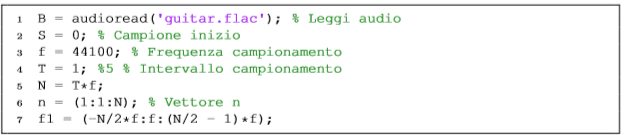
\includegraphics[width=.8\textwidth]{./images/cap4/acquisizione.png}
\end{figure}

\section{Periodogramma Semplice}
Una volta acquisito correttamente $x(n)$ è possibile valutarne il periodogramma 
semplice mediante la definizione e la libreria di MATLAB \textit{ftt()}:

\begin{minipage}[t]{.25\textwidth}
	\vspace*{.75cm}
	\begin{equation*}
	P_X (k) = \frac{|X(k)|^2}{N}
	\end{equation*}
\end{minipage}
\hfill
\begin{minipage}[t]{.7\textwidth}
	\begin{figure}[H]
		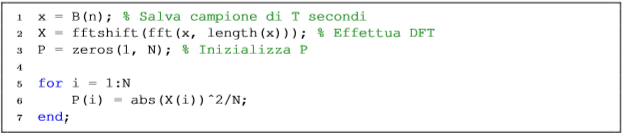
\includegraphics[width=\textwidth]{./images/cap4/ifft.png}
	\end{figure}
\end{minipage}

\bigskip

Una volta calcolati i periodogrammi per uno e cinque secondi di registrazione, 
è possibile disegnarli mediante il comando \textit{plot()} di MATLAB e 
valutarne le differenze:

\begin{minipage}[t]{.45\textwidth}
	\begin{figure}[H]
		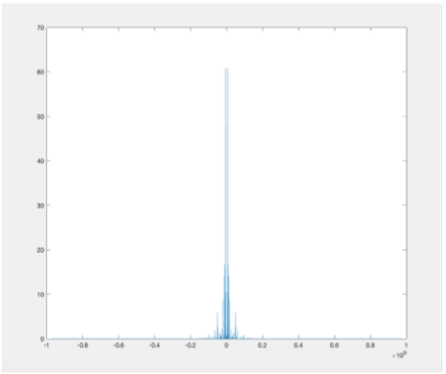
\includegraphics[width=\textwidth]{./images/cap4/per1s.png}
		\caption{Periodogramma per 1 secondo di registrazione.}
	\end{figure}
\end{minipage}
\hfill
\begin{minipage}[t]{.45\textwidth}
	\begin{figure}[H]
		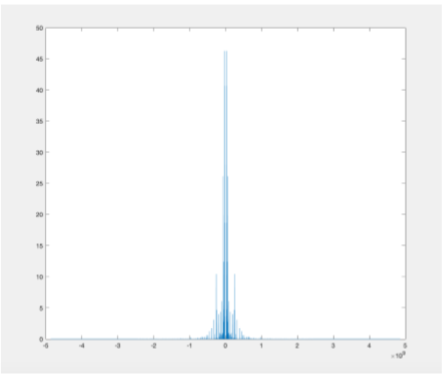
\includegraphics[width=\textwidth]{./images/cap4/per5s.png}
		\caption{Periodogramma per 5 secondi di registrazione.}
	\end{figure}
\end{minipage}

Si può affermare che il periodogramma valutato su un intervallo di cinque 
secondi risulta più fitto e mostra un maggior numero di contenuto 
in frequenza.

%-------------------------------------------------------------------------------

\section{Periodogramma di Barlett}
Come osservato nel punto precedente, il periodogramma semplice ha elevata 
risoluzione in frequenza ma è “rumoroso”. Una tecnica per ridurre il rumore è 
eseguire il cosiddetto periodogramma di Bartlett, ottenuto dividendo la 
sequenza x(n) in M intervalli disgiunti di $N/M$ campioni 
ciascuno, calcolando il periodogramma di ciascuna sottosequenza e 
mediando il risultato.
\begin{minipage}[t]{.35\textwidth}
	\begin{figure}[H]
		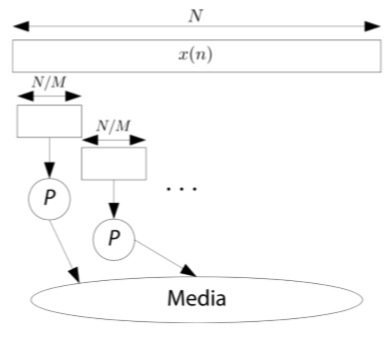
\includegraphics[width=\textwidth]{./images/cap4/barlett.png}
	\end{figure}
\end{minipage}
\hfill
\begin{minipage}[t]{.55\textwidth}
	\vspace*{2cm}
	\begin{equation*}
		P_X(k) = \frac{1}{M} \sum^{M-1}_{i=0} \frac{|X^{(i)}(k)|^2}{N/M}
	\end{equation*}
\end{minipage}

\bigskip

dove $X_{(i)}(k)$ è la DFT dell'i-esimo intervallo $x(n)$. Una volta 
acquisito correttamente x(n) è possibile valutarne il periodogramma di 
Bartlett mediante la definizione per valori $M = 10, 50, 100$.

\begin{figure}[H]
	\centering
	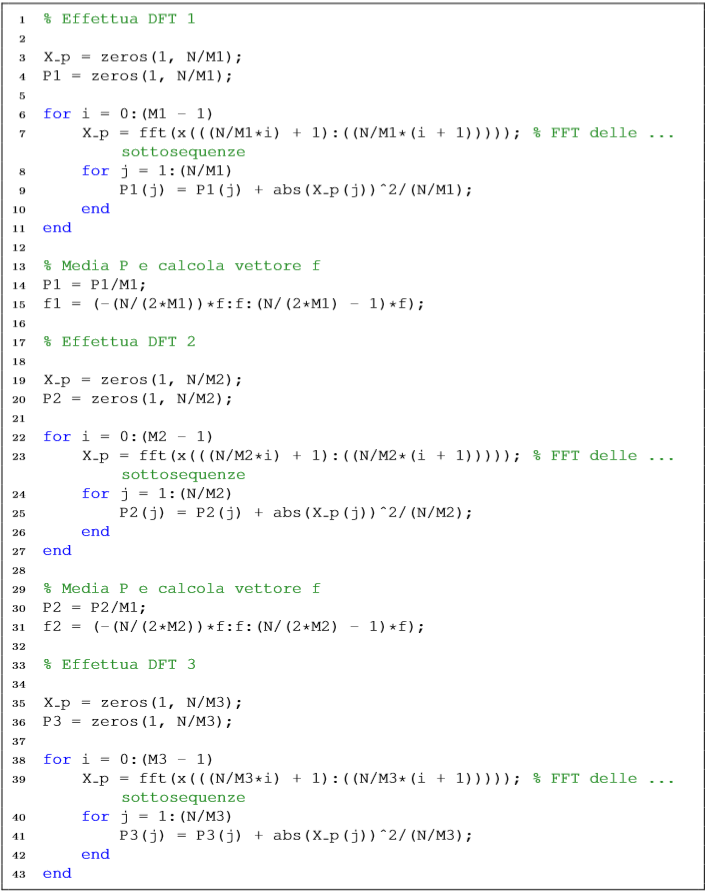
\includegraphics[width=.8\textwidth]{./images/cap4/mat_barlett.png}
\end{figure}

Una volta calcolati i periodogrammi per uno e cinque secondi di registrazione, 
è possibile disegnarli mediante il comando \textit{plot()} di MATLAB e 
valutarne le differenze:

\begin{minipage}[t]{.45\textwidth}
	\begin{figure}[H]
		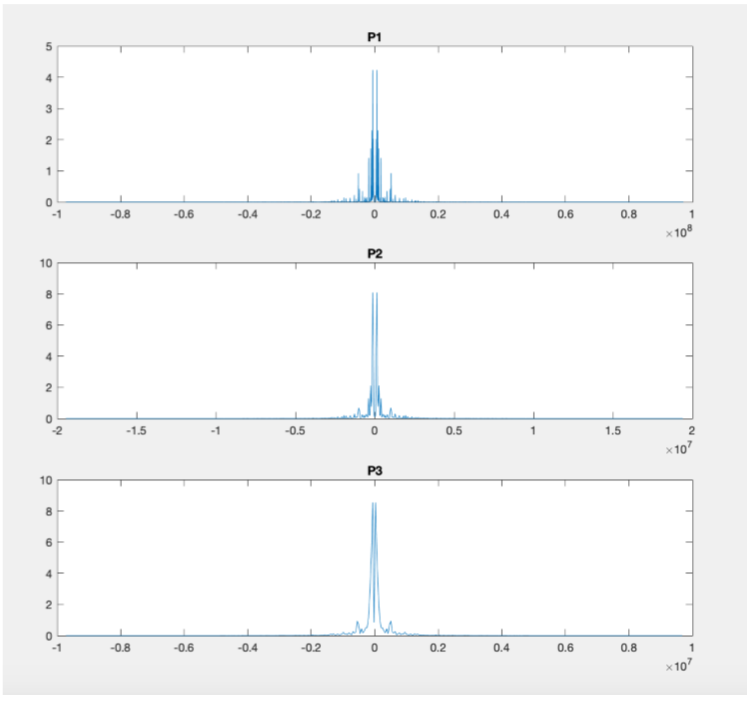
\includegraphics[width=\textwidth]{./images/cap4/barlett1s.png}
		\caption{Periodogramma di Barlett per 1 secondo di registrazione.}
	\end{figure}
\end{minipage}
\hfill
\begin{minipage}[t]{.45\textwidth}
	\begin{figure}[H]
		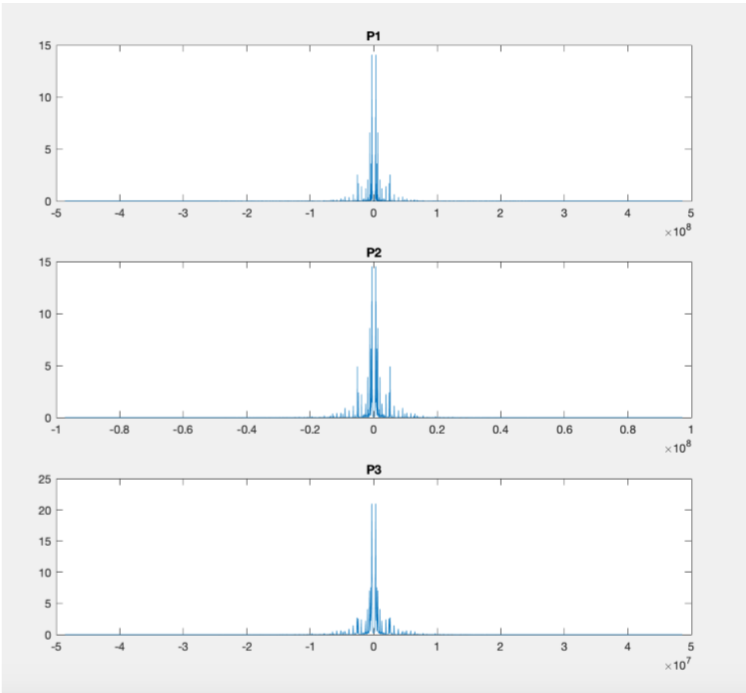
\includegraphics[width=\textwidth]{./images/cap4/barlett5s.png}
		\caption{Periodogramma di Barlett per 5 secondi di registrazione.}
	\end{figure}
\end{minipage}

%-------------------------------------------------------------------------------

\section{Periodogramma di Welch}
Come visto al punto precedente, il periodogramma di Bartlett consente di ridurre 
il “rumore” sulla stima di densità spettrale di potenza, riducendone al contempo 
la risoluzione. Una tecnica più avanzata è il periodogramma di Welch. Rispetto al 
periodogramma di Bartlett, introduce le seguenti modifiche:

\begin{itemize}
	\item Le sotto-sequenze su cui si calcola il periodogramma non sonodisgiunte 
	ma sono sovrapposte del 50\%.

	\begin{figure}[H]
		\centering
		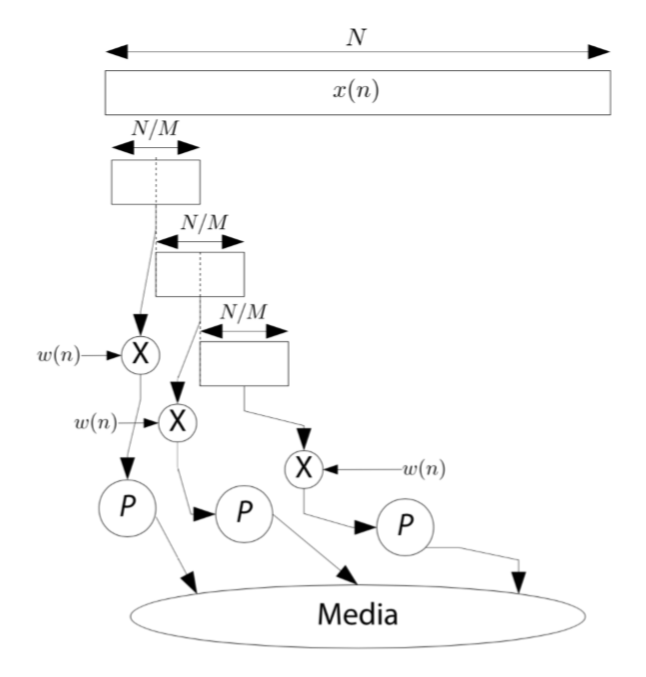
\includegraphics[width=.5\textwidth]{./images/cap4/welch_schema.png}
	\end{figure}

	\item  Prima di eseguire la DFT, ogni sotto-sequenza viene moltiplicata per 
	una funzione $w(n)$ chiamata finestra di Hamming:
	
	\begin{equation*}
		w(n) = \alpha - \beta cos(\frac{2 \pi n}{N/M -1})
	\end{equation*}	
\end{itemize}

La funzione è presente nella libreria di MATLAB sotto il nome di \textit{hamming()}.
Una volta acquisito correttamente x(n) è possibile valutarne il periodogramma di 
Welch mediante la definizione per valori $M = 10, 50, 100$ come fatto per il 
periodogramma di Bartlet.

\begin{figure}[H]
	\centering
	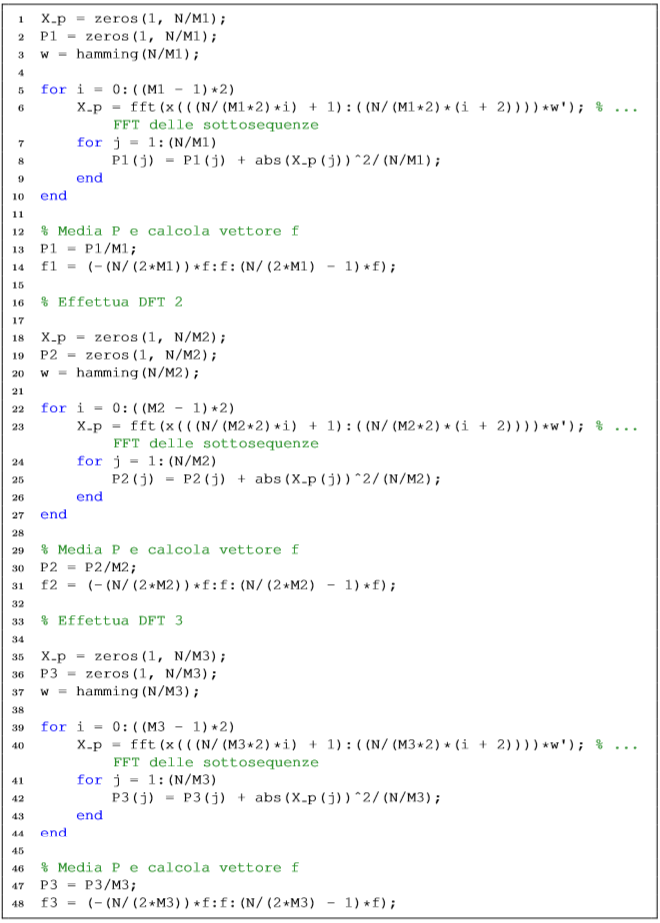
\includegraphics[width=0.7\textwidth]{images/cap4/matlab_welch}
\end{figure}

Eseguendo il periodogramma di Welch della sequenza x(n) usando gli stessi parametri 
usati per il periodogramma di Bartlett `e possibile mettere a confronto i risultati 
ottenuti.

\begin{figure}[H]
	\centering
	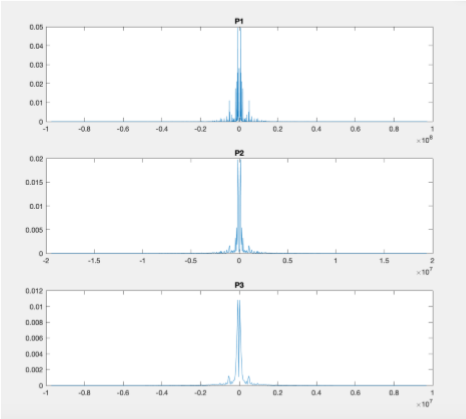
\includegraphics[width=0.7\textwidth]{images/cap4/plot_welch}
\end{figure}


Si nota una riduzione del disturbo nella variazione del periodogramma semplice, 
senza una eccessiva perdita dell’informazione in frequenza.

